\documentclass[twocolumn]{jsarticle}
\usepackage[dvipdfmx]{graphicx}
\usepackage{mathrsfs,calligra,calrsfs,url,bm,here,caption}
% \captionsetup[table]{labelsep=period,justification=raggedright, singlelinecheck=off}
\usepackage{aic2022}
\title{AICカンファレンス ポスター発表 要旨}
\author{西川誠人$^1$,勝又圭$^2$,好田駿成$^3$}
\affiriation{$^1$慶應義塾大学大学院理工学研究科\\$^2$慶應義塾大学理工学部情報工学科\\$^3$慶應義塾大学経済学部}
\abst{\\
昨今,ビジネスにおいてビッグデータを活用する取り組みが広く行われている.一方で,データ活用のためには相応のデータ基盤が必要になるため,
人材やノウハウの無い企業においてはデータ活用が遅れている.この現状に対し,企業にデータ活用プラットフォームを提供するサービスが生まれている.
我々は,このようなサービスの1つである,Databricksについて調査し,AICの講習会を行うことを目的に活動している.
本ポスターではこれまで我々が行ってきた調査内容についての発表を行う.
}
\keywords{Databricks, Machine Learning, Datawarehouse, AI, Open Source}
\begin{document}
\maketitle
\section{研究背景・目的}
2022年度のAIC新設のプロジェクトとして,新しいAI/Data Science PlatformであるDatabricksの調査・評価プロジェクトが2022年6月からスタートした。
Databricksとはデータの収集・蓄積から分析・機械学習モデル開発並びに運用を一気通貫・効率的かつ安価に行うことができるオープンソースの統合プラットフォーム\cite{databricksHP}である。
機械学習・AIが注目される昨今だが、情報インフラ構築の難易度やノウハウの欠如からデータ活用ができていない企業も多く、機械学習エンジニアの雇用・分析環境の構築の観点から機械学習の大規模な活用は大企業にとどまることがほとんどである。
今回の調査対象であるDatabricksを提供するDatbricks社はデータとAIの民主化を掲げ、機械学習等のデータ活用を大企業以外にも活用できるようにノウハウを持たない企業におけるデータ活用を推進している。
DatabricksはGartnerの2022年「クラウドデータベース管理システム(CDBMS)部門のマジック・クアドラント」において、2年連続でリーダーの1社\cite{Gartner}として位置付け今後のDe Fact Standard化が期待されている。
そんなDatabricksについて学生視点から分析を行い、慶應義塾大学内での活用可能性やDatabricksを学ぶことの意義を評価することが本プロジェクトの目的である。
\section{方法}
本プロジェクト実施にあたりDatabricksの提供手法の一つであるDatabricks On AWSを使用した。他のクラウドプラットフォームとしてGoogle Cloud Platform, Microsoft Azure等が挙げられるが、
実際にDatabricksが活用されている企業の中で一番使われていること、Databricks社が2022年8月に実施したDatbricks Hands Onにて使用されていたことなどからAWSを選択した。\par 
調査方法は主に以下の手順によって実施した。
\begin{enumerate}
  \item Databricks社の提供するHands On への参加
  \item Databricks社が提供する学習コンテンツDatabricks Learningを用いた学習の実施
  \item オープンデータを用いた自由なDatabricksのデータ分析の実施
  \item 他の類似サービスとの比較・優位性の調査
\end{enumerate}
以上の手順によりDatabricksの学習コスト、他のプラットフォームを使用した際と比較したデータ分析のしやすさを評価した。
\vspace{-6zh}
\section{Databricksについて}
\vspace{-3.5zh}
\subsection{サービスアーキテクチャ}
% \vspace{-1zh}
\subsubsection{レイクハウスとは}
Databricksでは新たなデータ活用プラットフォームの形としてレイクハウスを提案している。
レイクハウスとは一般的に企業などで構造化データを用いる際に活用されるデータウェアハウスと多様なデータを単一のシステムで活用するためのデータレイクそれぞれの利点を組み合わせたアーキテクチャである。
一般に古くから用いられるデータウェアハウスは近年の機械学習の発達により活用が促進されている画像や音声などの非構造化データの格納には適しておらず、データレイクはトランザクション・データ品質の保証等に適していないという課題があった。
これらの課題を解決するのがレイクハウスであり、データウェアハウスと同様のデータ構造とデータ管理能力を搭載している他、データレイクのメリットである低コストなストレージへの直接アクセスを実現している。
構造化データは勿論、非構造化データ等のさまざまなデータタイプが格納できるほか、トランザクションやBI、様々な言語が同一のノートブックで使用できるなど他のプラットフォームと比較した優位性があるといえる。
DatabricksにおけるレイクハウスプラットフォームはFig.\ref{lakehouse}のように構成されている。DatabricksでレイクハウスはDelta Lake と呼ばれるOSSで実現されており、Databricksの各種サービス・機能はDelta Lakeをベースとして提供されている。\par
\begin{figure}[H]
  \centering
  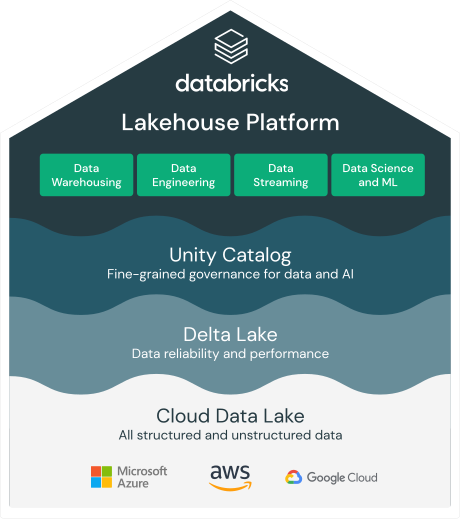
\includegraphics[width=6cm]{./image/Marketecture.png}
  \caption{レイクハウスプラットフォーム概略図}
  \label{lakehouse}
  \title
\end{figure}
\subsubsection{インフラ}
Databricksで用いられるインフラ構築は一括で各クラウドプラットフォームをもとに行われている。DatabrickではMicrosoft Azure、Amazon Web Servbices、 Google Cloud Platformの3種のクラウドに対応しており、それぞれのインフラ管理についてもDatabricks専用のGUIによって管理可能である。
ノウハウが少ない中小企業での活用を目的としていることもあり、Databricksに必要な機能に絞った構成となっており、各クラウドから自力で環境構築するより容易であり学習コストも低い。
\subsection{主要機能}
Databricksでは主にData Science \& Engineering、Databricks SQL、Databricks MLの3つの機能から構成されている。
\subsubsection{Data Science \& Engineering}
Data Science \& Engineeringはデータの取得・加工を目的とした
\subsubsection{Databricks SQL}
\subsubsection{Databricks ML}
\section{調査結果}
\subsection{Databricksの強み}
\subsection{他プラットフォームとの比較}
\subsection{大学内での使用可能性評価}
% \subsection{}
\section{今後の展開}
\section{結論}
本プロジェクトによりDatabricks社により提供されているDatabricksというデータ活用プラットフォームの有用性を評価することができた。ビジネス文脈で使用される機能を多く備えたツールであるという側面は理解した上で、
機械学習を使用することを目的として研究や学習用途で学生が使う有用性は大いに認められるだろう。AIC DatabricksプロジェクトとしてDatabricksの慶應義塾大学における普及・De Falcto Standard化を促進するため、Databricksに関する
授業提供を実施する。学生に機械学習が容易に活用できるという選択肢を提示することにより今後の慶應義塾大学での研究・学習における機械学習の活用が促進されることで未来の研究にポジティブに寄与してゆきたい。

\begin{thebibliography}{9}
  \bibitem{databricksHP} S. Yagami, Science, \textbf{393}, 113--117 (1998).
  \bibitem{Gartner} S. Yagami \textit{et al}., Proc. IEEE \textbf{52}, 284--290 (2013).
  \bibitem{QuickStartGuide}  クイックスタートガイド
  \bibitem{about_databricks} \url{https://learn.microsoft.com/ja-jp/azure/databricks/scenarios/what-is-azure-databricks-ws}
  \bibitem{}
  \end{thebibliography}
\end{document}
%\label{lakehouse} $\url{https://www.databricks.com/jp/product/data-lakehouse}$]
